% !TEX program = xelatex
% 北京理工大学专用 Beamer 模板（非官方）
% 修改下方“演示元信息”即可开始；每个 frame 都可复制复用。
\documentclass[aspectratio=169,10pt]{beamer}

% ---------- 基础包 ----------
\usepackage{xeCJK}
\usepackage{fontspec}
\usepackage{graphicx}
\usepackage{booktabs}
\usepackage{tabularx}
\usepackage{array}
\usepackage{ragged2e}
\usepackage{tikz}
\usepackage{pifont}
\usepackage{amsmath}
\usetikzlibrary{arrows.meta,calc,positioning,shapes.geometric}

% ---------- 字体 ----------
% macOS 默认使用苹方；Linux/Windows 可将字体名改为系统中的中文字体。
\setmainfont{Arial}
\setsansfont{Arial}
\setCJKmainfont{PingFang SC}
\setCJKsansfont{PingFang SC}
\renewcommand{\familydefault}{\sfdefault}

% ---------- 演示元信息：从这里开始替换 ----------
\newcommand{\PresentationTitle}{北京理工大学专用 Beamer 模板}
\newcommand{\PresentationSubtitle}{用清晰结构讲好一个学术故事}
\newcommand{\PresentationAuthor}{姓名 / 团队名称}
\newcommand{\PresentationAffiliation}{北京理工大学 · 学院 / 课题组}
\newcommand{\PresentationDate}{\today}
\newcommand{\PresentationTopic}{学术汇报 · 课程展示 · 项目答辩}

% ---------- 品牌色 ----------
\definecolor{BITBlue}{RGB}{0,63,104}
\definecolor{BITBlueLight}{RGB}{229,241,248}
\definecolor{BITRed}{RGB}{168,35,54}
\definecolor{BITGreen}{RGB}{24,120,74}
\definecolor{BITGold}{RGB}{183,101,19}
\definecolor{Ink}{RGB}{40,49,55}
\definecolor{Muted}{RGB}{105,121,132}
\definecolor{Line}{RGB}{210,221,227}
\definecolor{Panel}{RGB}{246,249,250}

\hypersetup{colorlinks=false}
\setbeamercolor{normal text}{fg=Ink,bg=white}
\setbeamercolor{structure}{fg=BITBlue}
\setbeamertemplate{navigation symbols}{}
\setbeamersize{text margin left=2.55cm,text margin right=.72cm}
\setlength{\parskip}{.2em}
\renewcommand{\arraystretch}{1.18}

% ---------- 文字与组件 ----------
\newcommand{\bword}[1]{\textbf{\textcolor{BITBlue}{#1}}}
\newcommand{\rword}[1]{\textbf{\textcolor{BITRed}{#1}}}
\newcommand{\gword}[1]{\textbf{\textcolor{BITGreen}{#1}}}
\newcommand{\smallsource}[1]{{\scriptsize\color{Muted}#1}}
\newcommand{\mycheck}{\textcolor{BITGreen}{\ding{51}}}
\newcommand{\tightlist}{\setlength\itemsep{.12cm}\setlength\parsep{0pt}\setlength\topsep{.05cm}}
\newcolumntype{Y}{>{\RaggedRight\arraybackslash}X}
\newcolumntype{L}[1]{>{\RaggedRight\arraybackslash}p{#1}}

\newcommand{\InsightBox}[3]{%
\begin{tikzpicture}\node[draw=#1!65,fill=#1!8,rounded corners=3pt,inner sep=6pt,text width=#2,align=left]{#3};\end{tikzpicture}}
\newcommand{\MetricCard}[3]{%
\begin{tikzpicture}\node[draw=Line,fill=white,rounded corners=3pt,minimum width=3.1cm,minimum height=1.65cm,align=center]{\fontsize{21}{24}\selectfont\bfseries\color{#1}#2\\[-1pt]{\scriptsize\color{Muted}#3}};\end{tikzpicture}}
\newcommand{\PhotoCard}[3]{%
\begin{tikzpicture}\node[inner sep=0pt,rounded corners=3pt] (photo) {\includegraphics[width=#1,height=#2,keepaspectratio]{#3}};\end{tikzpicture}}

% ---------- 背景、侧栏与页脚 ----------
\newcommand{\NavItem}[2]{\ifnum\value{section}=#1\relax{\bfseries\color{BITBlue}#2}\else{\color{Muted}#2}\fi}
\newcommand{\PageChrome}{%
\begin{tikzpicture}[remember picture,overlay]
  \fill[white] (current page.south west) rectangle (current page.north east);
  \node[anchor=south,opacity=.10,inner sep=0pt] at (current page.south) {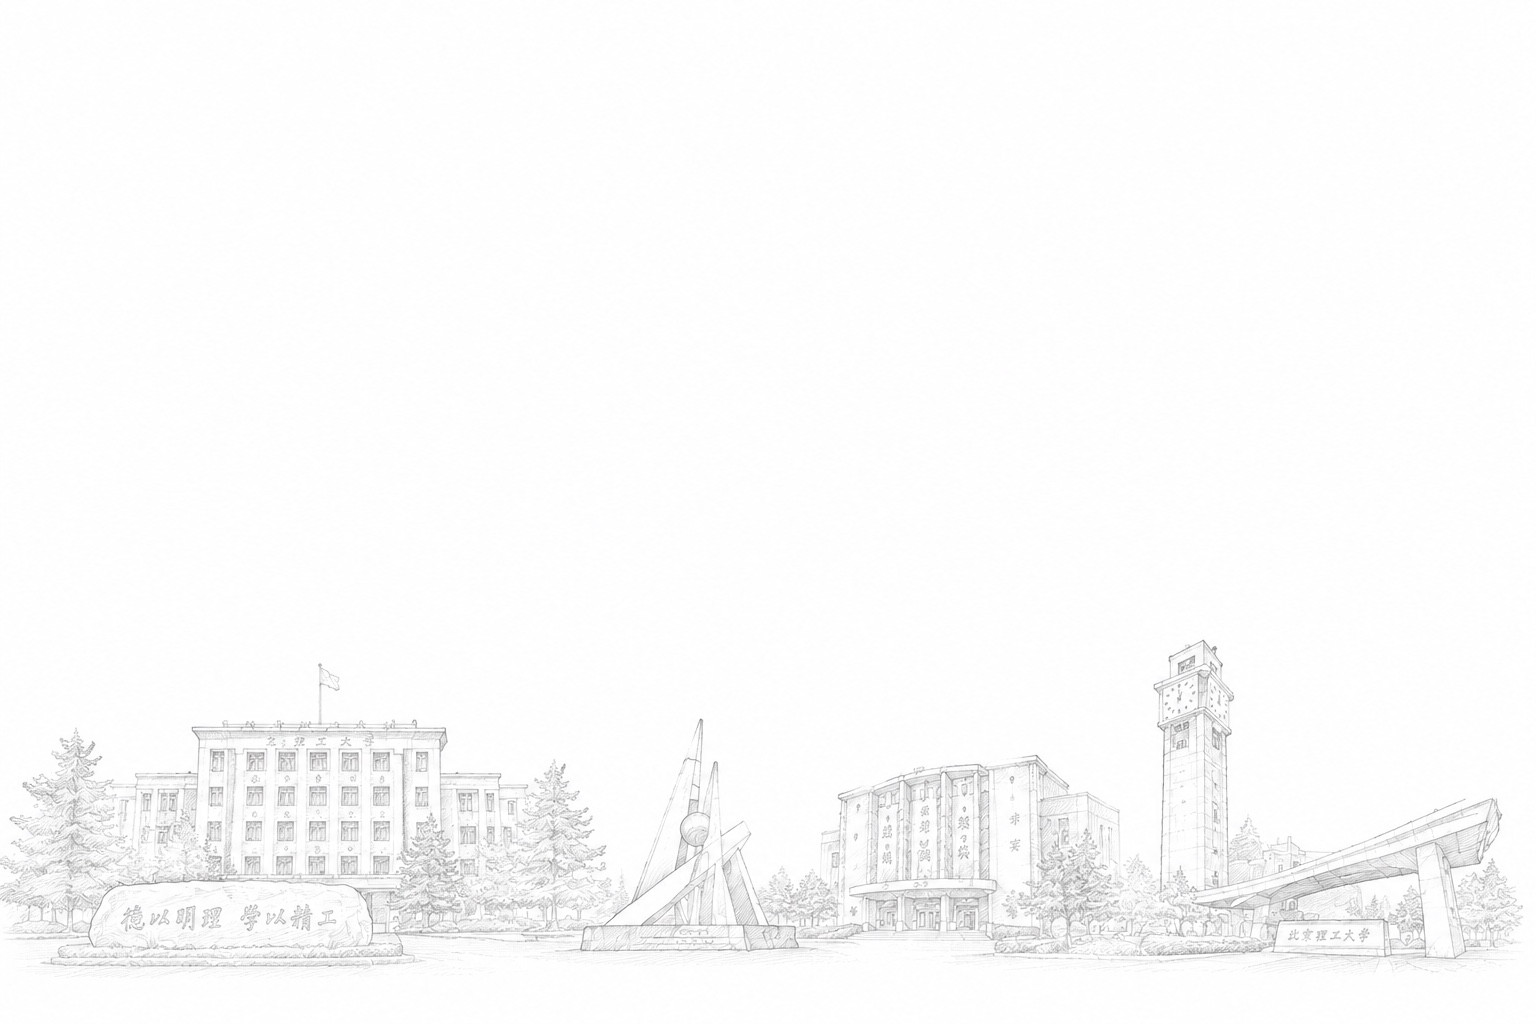
\includegraphics[width=\paperwidth]{assets/bit_campus_background.jpeg}};
  \node[anchor=center,opacity=.14,inner sep=0pt] at ([xshift=6.5cm,yshift=-.65cm]current page.center) {
\includegraphics[width=7.2cm]{assets/bit_green_logo.png}};
  \fill[Panel] (current page.north west) rectangle ([xshift=2.26cm]current page.south west);
  \draw[Line,line width=.3pt] ([xshift=2.26cm]current page.north west) -- ([xshift=2.26cm]current page.south west);
  \node[anchor=north,align=center,text width=1.72cm] at ([xshift=1.13cm,yshift=-.64cm]current page.north west) {\fontsize{7.6}{9.4}\selectfont\color{BITBlue}\PresentationTopic};
  \node[anchor=north,align=center,text width=1.75cm] at ([xshift=1.13cm,yshift=-1.55cm]current page.north west) {\fontsize{8.5}{10}\selectfont\color{Ink}\PresentationAuthor};
  \node[anchor=west,text width=1.75cm] at ([xshift=.28cm,yshift=-3.20cm]current page.north west) {\fontsize{9.8}{16}\selectfont\NavItem{1}{01\quad 开场与问题}};
  \node[anchor=west,text width=1.75cm] at ([xshift=.28cm,yshift=-4.13cm]current page.north west) {\fontsize{9.8}{16}\selectfont\NavItem{2}{02\quad 证据与洞察}};
  \node[anchor=west,text width=1.75cm] at ([xshift=.28cm,yshift=-5.06cm]current page.north west) {\fontsize{9.8}{16}\selectfont\NavItem{3}{03\quad 路径与行动}};
  \node[anchor=west,text width=1.75cm] at ([xshift=.28cm,yshift=-5.99cm]current page.north west) {\fontsize{9.8}{16}\selectfont\NavItem{4}{04\quad 总结与致谢}};
  \node[anchor=north east,inner sep=0pt] at ([xshift=-.30cm,yshift=-.16cm]current page.north east) {
\includegraphics[width=2.92cm]{assets/bit_logo.pdf}};
\end{tikzpicture}%
}
\setbeamertemplate{background}{\PageChrome}
\setbeamertemplate{frametitle}{%
\begin{tikzpicture}[remember picture,overlay]
\node[anchor=west,text width=10.5cm] at ([xshift=2.66cm,yshift=-.66cm]current page.north west) {\fontsize{13}{15.4}\selectfont\bfseries\color{BITBlue}\insertframetitle};
\draw[Line,line width=.45pt] ([xshift=2.66cm,yshift=-1.13cm]current page.north west) -- ([xshift=-.55cm,yshift=-1.13cm]current page.north east);
\end{tikzpicture}\vspace{1.06cm}}
\setbeamertemplate{footline}{\begin{tikzpicture}[remember picture,overlay]
\node[anchor=south west] at ([xshift=2.67cm,yshift=.14cm]current page.south west) {\scriptsize\color{Muted}北京理工大学专用 Beamer 模板 · \PresentationTopic};
\node[anchor=south east] at ([xshift=-.35cm,yshift=.14cm]current page.south east) {\scriptsize\color{Muted}\insertframenumber / \inserttotalframenumber};
\end{tikzpicture}}

\newcommand{\TitleChrome}{%
\begin{tikzpicture}[remember picture,overlay]
\fill[white] (current page.south west) rectangle (current page.north east);
\node[anchor=south,opacity=.28,inner sep=0pt] at (current page.south) {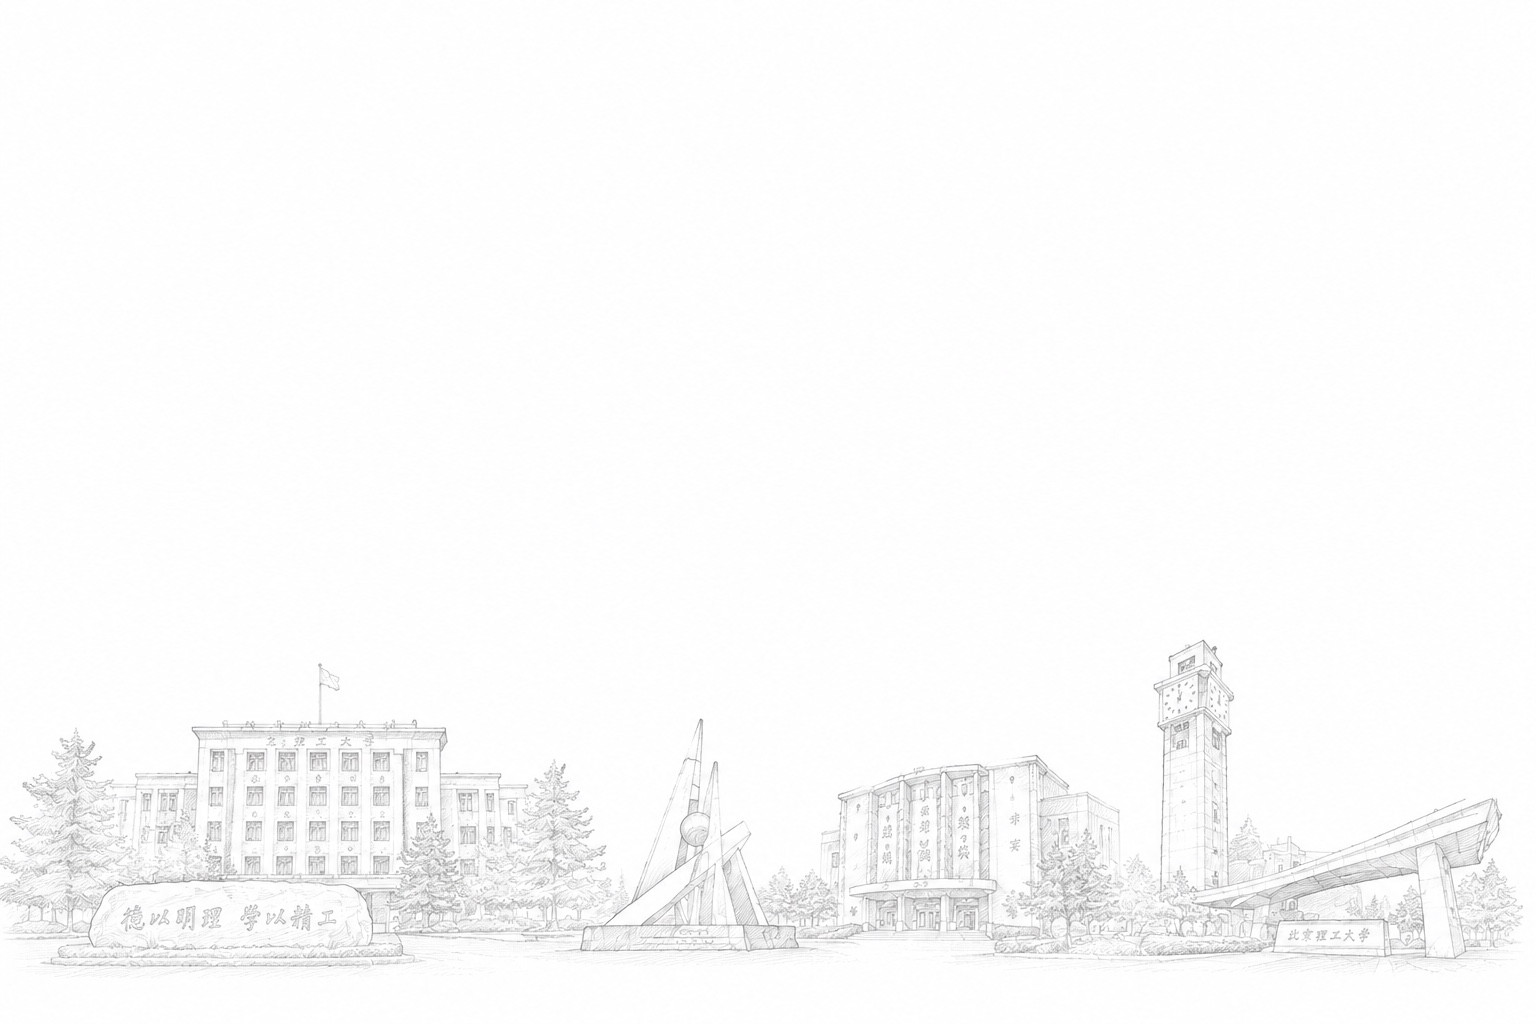
\includegraphics[width=\paperwidth]{assets/bit_campus_background.jpeg}};
\node[anchor=center,opacity=.43,inner sep=0pt] at ([xshift=5.7cm,yshift=-.10cm]current page.center) {
\includegraphics[width=8.0cm]{assets/bit_green_logo.png}};
\node[anchor=north east,inner sep=0pt] at ([xshift=-.46cm,yshift=-.38cm]current page.north east) {
\includegraphics[width=3.18cm]{assets/bit_logo.pdf}};
\draw[BITBlue,line width=1.1pt] ([xshift=1.2cm,yshift=-1.22cm]current page.north west) -- ([xshift=-1.2cm,yshift=-1.22cm]current page.north east);
\end{tikzpicture}%
}

\begin{document}

% ---------- 封面 ----------
{\setbeamertemplate{background}{\TitleChrome}\setbeamertemplate{footline}{}
\begin{frame}[plain]\vspace{1.13cm}\begin{center}
{\fontsize{23}{27}\selectfont\bfseries\color{BITBlue}\PresentationTitle\par}
\vspace{.32cm}{\Large\color{Ink}\PresentationSubtitle\par}
\vspace{.84cm}\begin{tabular}{rl}\toprule
汇报人 & \PresentationAuthor\\
单位 & \PresentationAffiliation\\
日期 & \PresentationDate\\\bottomrule
\end{tabular}\end{center}\end{frame}}

\section{开场与问题}
\begin{frame}[t]{一页讲清：你的研究 / 项目为何重要}
\small
\InsightBox{BITBlue}{11.25cm}{\textbf{把结论放在最前面。}\quad 用一句完整的话定义本次汇报最希望听众记住的观点，例如：\bword{我们发现了一个重要问题，并提出了一条可验证、可执行的解决路径。}}
\vspace{.30cm}\begin{columns}[T,onlytextwidth]
\begin{column}{.47\textwidth}\begin{itemize}\tightlist
\item \bword{背景：}用 1--2 个事实说明场景与紧迫性。
\item \bword{缺口：}指出现有做法、研究或产品尚未解决什么。
\item \bword{目标：}明确本次要回答的问题或要实现的结果。
\end{itemize}\end{column}
\begin{column}{.49\textwidth}\centering
\begin{tikzpicture}[node distance=.45cm]
\tikzset{routebox/.style={draw=BITBlue!60,fill=white,rounded corners=3pt,minimum width=4.3cm,minimum height=.63cm,align=center}}
\node[routebox] (a) {现实挑战 / 学术问题};\node[routebox,below=of a] (b) {关键证据与核心洞察};\node[routebox,below=of b,draw=BITGreen!70,fill=BITGreen!8] (c) {可落地的解决方案};
\draw[-{Latex[length=2mm]},BITRed,line width=.8pt] (a)--(b);\draw[-{Latex[length=2mm]},BITGreen,line width=.8pt] (b)--(c);
\end{tikzpicture}\end{column}\end{columns}
\end{frame}

\begin{frame}[t]{汇报结构：让听众始终知道你在哪里}
\centering\vspace{.55cm}
\begin{tikzpicture}[node distance=.46cm]
\tikzset{road/.style={draw=BITBlue!60,fill=white,rounded corners=4pt,minimum width=2.25cm,minimum height=1.45cm,align=center}}
\node[road] (a) {\color{BITRed}\bfseries 01\\[2pt]\color{Ink}问题定义};
\node[road,right=of a] (b) {\color{BITBlue}\bfseries 02\\[2pt]\color{Ink}证据分析};
\node[road,right=of b] (c) {\color{BITGreen}\bfseries 03\\[2pt]\color{Ink}解决路径};
\node[road,right=of c] (d) {\color{BITGold}\bfseries 04\\[2pt]\color{Ink}总结行动};
\draw[-{Latex[length=2mm]},BITBlue!75,line width=1pt] (a)--(b);\draw[-{Latex[length=2mm]},BITBlue!75,line width=1pt] (b)--(c);\draw[-{Latex[length=2mm]},BITBlue!75,line width=1pt] (c)--(d);
\end{tikzpicture}
\vspace{.76cm}\InsightBox{BITRed}{10.4cm}{\centering\textbf{版式提示：}章节页不必堆砌目录。用一条有方向的叙事线，让每个章节都回答一个更具体的问题。}
\end{frame}

\section{证据与洞察}
\begin{frame}[t]{数据页：用一个主结论统领所有数字}
\centering\vspace{.06cm}
\MetricCard{BITBlue}{72\%}{关键指标 A}\hspace{.28cm}\MetricCard{BITRed}{3.6×}{关键指标 B}\hspace{.28cm}\MetricCard{BITGreen}{18}{样本 / 场景数}
\vspace{.35cm}\begin{columns}[T,onlytextwidth]
\begin{column}{.54\textwidth}\small
\bword{图表标题应写成结论：}某项指标在关键节点后显著改善。\\[4pt]
\begin{tikzpicture}[x=.9cm,y=.65cm]
\draw[->,BITBlue] (0,0)--(6,0) node[right,black]{时间};\draw[->,BITBlue] (0,0)--(0,4) node[above,black]{指标};
\foreach \y in {1,2,3}{\draw[Line] (0,\y)--(5.65,\y);}
\draw[BITRed,line width=1.3pt] plot coordinates {(0.45,.72) (1.3,1.08) (2.15,1.34) (3,2.06) (3.85,2.58) (4.7,3.18) (5.5,3.52)};
\foreach \x/\y in {.45/.72,1.3/1.08,2.15/1.34,3/2.06,3.85/2.58,4.7/3.18,5.5/3.52}{\fill[BITRed](\x,\y)circle(1.5pt);}
\node[align=center,fill=BITBlueLight,draw=BITBlue!40,rounded corners,inner sep=3pt] at (4.65,.58) {转折点\\在此解释};
\end{tikzpicture}\end{column}
\begin{column}{.42\textwidth}\small
\InsightBox{BITGreen}{4.75cm}{\textbf{读图结论}\par 数据不是装饰；先写出趋势的含义，再保留支撑这个结论的最少数字。}
\vspace{.2cm}\InsightBox{BITGold}{4.75cm}{\textbf{数据来源}\par 在此填写：数据库 / 调研时间 / 样本范围。示例数值仅展示排版。}\end{column}\end{columns}
\end{frame}

\begin{frame}[t]{图文页：用真实场景让抽象观点可感知}
\begin{columns}[T,onlytextwidth]
\begin{column}{.53\textwidth}\vspace{.10cm}
\PhotoCard{6.1cm}{4.7cm}{assets/bit_campus_background.jpeg}\\[-1pt]
\smallsource{图片：模板随附的校园背景；使用时可替换为项目现场、实验装置或调研照片。}\end{column}
\begin{column}{.43\textwidth}\small
\InsightBox{BITBlue}{4.85cm}{\textbf{场景化表达}\par 将一张图片与一个具体事实配对：它告诉听众\rword{什么正在发生}，又为什么值得关注。}
\vspace{.2cm}\begin{itemize}\tightlist
\item 图片只承担一个叙事角色。
\item 用 2--3 个短句解释观察到的现象。
\item 避免把整段材料塞进图片旁。
\end{itemize}\vspace{.1cm}
\InsightBox{BITRed}{4.85cm}{\textbf{可替换区域}\par \texttt{assets/bit\_campus\_background.jpeg} 可直接改为你的图片路径。}\end{column}\end{columns}
\end{frame}

\section{路径与行动}
\begin{frame}[t]{方案页：从洞察走向可执行的行动}
\centering\vspace{.18cm}
\begin{tikzpicture}[node distance=.42cm]
\tikzset{phase/.style={draw=BITBlue!55,fill=white,rounded corners=4pt,minimum width=2.48cm,minimum height=1.65cm,align=center}}
\node[phase] (a) {\textcolor{BITRed}{\bfseries 发现}\\[-1pt]\scriptsize 定义问题与边界};
\node[phase,right=of a] (b) {\textcolor{BITBlue}{\bfseries 验证}\\[-1pt]\scriptsize 收集证据与测试};
\node[phase,right=of b] (c) {\textcolor{BITGreen}{\bfseries 实施}\\[-1pt]\scriptsize 配置资源与落地};
\node[phase,right=of c] (d) {\textcolor{BITGold}{\bfseries 评估}\\[-1pt]\scriptsize 追踪反馈与迭代};
\draw[-{Latex[length=2mm]},BITBlue,line width=.9pt] (a)--(b);\draw[-{Latex[length=2mm]},BITBlue,line width=.9pt] (b)--(c);\draw[-{Latex[length=2mm]},BITBlue,line width=.9pt] (c)--(d);
\end{tikzpicture}
\vspace{.48cm}\begin{columns}[T,onlytextwidth]
\begin{column}{.48\textwidth}\InsightBox{BITBlue}{5.35cm}{\textbf{建议 1：短期可启动}\par 说明最小行动、责任主体与完成时间。}\end{column}
\begin{column}{.48\textwidth}\InsightBox{BITGreen}{5.35cm}{\textbf{建议 2：中长期可扩展}\par 说明资源保障、评估指标与下一步协作。}\end{column}
\end{columns}\end{frame}

\section{总结与致谢}
\begin{frame}[t]{结论页：重复你最希望被记住的三件事}
\vspace{.15cm}\begin{columns}[T,onlytextwidth]
\begin{column}{.31\textwidth}\MetricCard{BITRed}{01}{用一句话重申问题}\end{column}
\begin{column}{.31\textwidth}\MetricCard{BITBlue}{02}{用一句话重申证据}\end{column}
\begin{column}{.31\textwidth}\MetricCard{BITGreen}{03}{用一句话重申行动}\end{column}\end{columns}
\vspace{.52cm}\InsightBox{BITBlue}{11.2cm}{\centering\Large\textbf{好的汇报不是信息的堆积，而是让听众看见：问题是什么、证据说明了什么、下一步可以做什么。}}\end{frame}

{\setbeamertemplate{background}{\TitleChrome}\setbeamertemplate{footline}{}
\begin{frame}[plain]\vspace{2.2cm}\begin{center}
{\fontsize{28}{32}\selectfont\bfseries\color{BITBlue}感谢聆听}\par\vspace{.38cm}
{\Large\color{Ink}Q \& A}\par\vspace{.48cm}{\small\color{Muted}\PresentationAffiliation}\end{center}\end{frame}}

\end{document}
